\documentclass{article}

\usepackage[top=2.54cm, left=2.54cm, right=2.54cm, bottom=2.54cm]{geometry}
\usepackage{amsmath}
\usepackage{graphicx}
\usepackage{booktabs}
\usepackage{hyperref}
\usepackage{multicol}
\hypersetup{colorlinks=true, urlcolor=blue,}
\usepackage[svgnames]{xcolor}


\begin{document}

\hrule
\begin{center}
\large {Quantum Harmonic Oscillator}\\ \large{and Hermite Polnomials}

\end{center}


\hrule
\vspace{1pt}
\hrule height 1pt

\vspace{.5cm}
\noindent\textbf{1  Introduction}
\vspace{.2cm}

\noindent The Schrodinger for a harmonic oscillator may be obtained by using
 the classical spring potential given by 

\begin{equation}
\label{eq:vx}
V(x)=\dfrac{1}{2}mw^2x^2
\end{equation}
where $m$ is the mass, $x$ is the position, and $w$ is the angular frequency
 given by 

\begin{equation}
\label{eq:w}
w=\sqrt{\frac{k}{m}}
\end{equation}
The Schrodinger equation with this form of potential is described by

\begin{equation}
\label{eq:Sch}
-\dfrac{h^2}{2m}\dfrac{d^2\Psi(x)}{dx^2}+V(x)\Psi(x) = E\Psi(x)
\end{equation}

Where V(x) is given by Eq. ~\eqref{eq:vx} Since the derivative of the
wavefunction must give back tthe square of $x$ plus a constant times the
original function, then the form
\begin{equation}
\label{eq:psiX}
\Psi(x)=Ce^{-ax^2/2}
\end{equation}
is suggested.
\\

Note that this form which is in a Gaussian form satisfies the requirement of going to zero at infinity, making it possible to normalize the wavefunction.  Substituting this function into the Schrodinger equation and fitting the boundary conditions leads to the ground state energy for the quantum harmonic oscillator given by
\begin{equation}
\label{eq:e0}
E_0= \dfrac{\hbar w}{2}
\end{equation}

The general solution to the Schrodinger equation leads to a sequence of 
evenly spaced energy levels characterized by a quantum number $n$ as shown in Fig. ~\ref{fig:energy}

\begin{figure}[ht]
\begin{center}
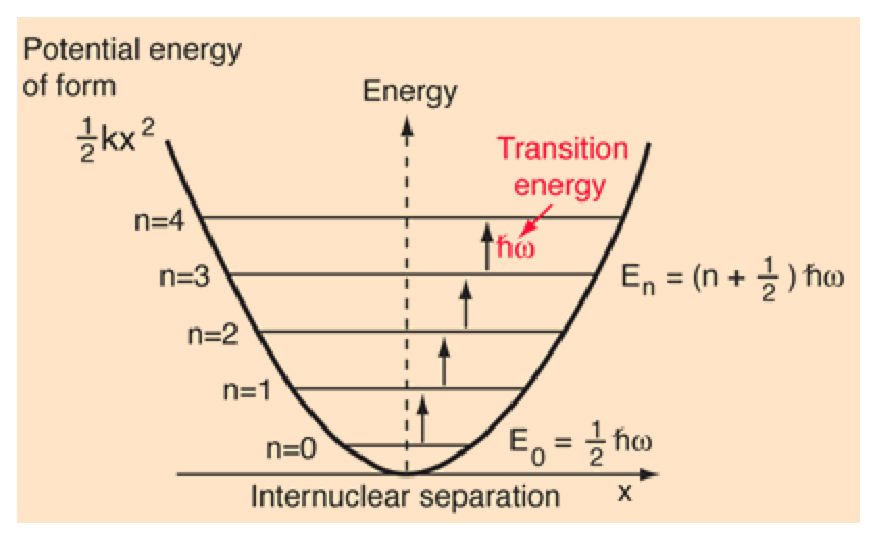
\includegraphics[scale=.6]{potwell.eps}
\caption{\label{fig:energy}Image Credit: \url{www.hyperphysics.com}}
\end{center}
\end{figure}
\clearpage
The wavefunctions for the quantum harmonic oscillator contain the Gaussian form which allows them to satisfy boundary conditions at infinity. In the wavefunction associated with a given value of the quantum number $n$, the Gaussian is multiplied by a polynomial of order $n$ called a \textbf{Hermite polynomial.}  The expressions are simplified by making the substitution

\begin{equation}
\label{eq:y}
y= \sqrt{ax}
\end{equation}

where $a = \dfrac{mw}{\hbar}$. The general formula for the normalized wavefunction is then

\begin{equation}
\label{eq:normalized}
\Phi(x)=(y)=(\frac{a}{\pi})^{\frac{1}{4}}\dfrac{1}{\sqrt{2^n n!}}H_n(y)e^\frac{-y^2}{2}
\end{equation}
Where $H_n(y)$ are the Hermite Polynomials.
\\
\\
\noindent\textbf{2  Solutions to the Schrodinger Equation}
\\
The Schrodinger equation for a harmonic oscillator may be solved to give the wavefunctions illustrated in
\begin{figure}[ht]
\begin{center}
\includegraphics[scale=.5,angle=-90]{hermite.ps}
\label{fig:hermite}
\end{center}
\end{figure}
\\
Figure 2: Solutions to the Schrodinger Equation for the first six energy states gives the normalized wave functions shown here.
\\
\\
The probability of finding the oscillator at any given value of x is the square of the wavefunction. Note that the wavefunctions for higher n have more “humps” within the potential well. This corresponds to a shorter wavelength and therefore by the deBroglie relationship they may be seen to have a higher momentum and therefore higher energy.
\\
\\
The most probable value of position for the lower states is very different from the classical harmonic oscillator where it spends more time near the end of its motion. But as the quantum number increases, the probability distribution becomes more like that of the classical oscillator.
\\
\\
When the Schrodinger equation for the harmonic oscillator is solved by a series method, the solutions contain this set of polynomials, named the Hermite polynomials. The values for n for the first six are shown in Table~\ref{table:table1}



\begin{center}
Table 1: blah
\\	

\begin{tabular}{l c r }	
\hline	
\hline
$n$	& $H_n(y)$   &          $E_n$\\	
\hline
0 & 1 & $\frac{1}{2}hw$\\
1 & 2$y^2$ - 2& $\frac{1}{2}hw$\\
2 & 4$y^2$- 2 & $\frac{3}{2}hw$\\
3 & 8$y^3$- 12$y$ & $\frac{5}{2}hw$\\
4 & 16$y^4$- 48$y^2$+12& $\frac{9}{2}hw$\\
5 & 32$y^5$ - 160$y^3$+120$y$ & $\frac{11}{2}hw$\\
\hline
\hline
\end{tabular}
\label{table:table1}
\end{center}

The wavefunctions for the quantum harmonic oscillator contain the Gaussian form which allows them to satisfy the necessary boundary conditions at infinity. In the wavefunction associated with a given value of the quantum number n, the Gaussian is multiplied by a polynomial of order n (the Hermite polynomials above) and the constants necessary to normalize the wavefunctions.
\end{document}



